\documentclass{article}
\usepackage{tikz}
\usetikzlibrary{arrows.meta, patterns}
\usepackage[margin=0.6in]{geometry}

\begin{document}

% One HIGH job (release t=0, period=30000us) sharing 4 cores with two LOW
% jobs (release t=0 and t=12500, period=12500us=80Hz) under the TDTA
% allocation. x-axis unit: 1 TikZ unit = 1000us. Derived by hand-simulating
% DAG-dependency-respecting, SCHED_FIFO-priority-preemptive execution from
% the actual core assignment TDTA produced for this scenario.
\begin{figure}[tb]
\centering
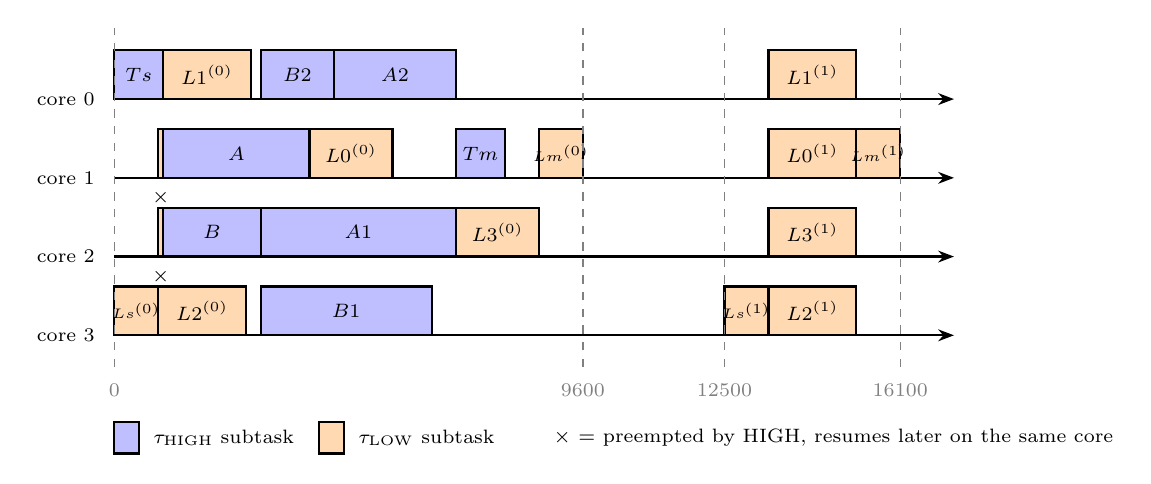
\begin{tikzpicture}[
    x=0.62cm, y=1cm,
    highblock/.style={fill=blue!25, draw=black, thick},
    lowblock/.style={fill=orange!30, draw=black, thick},
    tick/.style={font=\scriptsize},
    lbl/.style={font=\scriptsize}
]
    % ---- row baselines (y = 3: core0, 2: core1, 1: core2, 0: core3) ----
    \def\rowh{0.62}
    \foreach \y/\name in {3/core 0, 2/core 1, 1/core 2, 0/core 3} {
        \draw[-{Stealth[length=2mm]}, thick] (0,\y) -- (17.2,\y);
        \node[lbl, anchor=east] at (-0.2,\y) {\name};
    }

    % ================= core 0 =================
    \draw[highblock] (0,3)   rectangle ++(1,\rowh)   node[midway,lbl] {$Ts$};
    \draw[lowblock]  (1,3)   rectangle ++(1.8,\rowh) node[midway,lbl] {$L1^{(0)}$};
    \draw[highblock] (3,3)   rectangle ++(1.5,\rowh) node[midway,lbl] {$B2$};
    \draw[highblock] (4.5,3) rectangle ++(2.5,\rowh) node[midway,lbl] {$A2$};
    \draw[lowblock]  (13.4,3) rectangle ++(1.8,\rowh) node[midway,lbl] {$L1^{(1)}$};

    % ================= core 1 =================
    \draw[lowblock]  (0.9,2) rectangle ++(0.1,\rowh) node {};
    \draw[highblock] (1,2)   rectangle ++(3,\rowh)   node[midway,lbl] {$A$};
    \draw[lowblock]  (4,2)   rectangle ++(1.7,\rowh) node[midway,lbl] {$L0^{(0)}$};
    \draw[highblock] (7,2)   rectangle ++(1,\rowh)   node[midway,lbl] {$Tm$};
    \draw[lowblock]  (8.7,2) rectangle ++(0.9,\rowh) node[midway,font=\tiny] {$Lm^{(0)}$};
    \draw[lowblock]  (13.4,2) rectangle ++(1.8,\rowh) node[midway,lbl] {$L0^{(1)}$};
    \draw[lowblock]  (15.2,2) rectangle ++(0.9,\rowh) node[midway,font=\tiny] {$Lm^{(1)}$};
    \node[lbl, below=1pt] at (0.95,2) {\scriptsize$\times$};

    % ================= core 2 =================
    \draw[lowblock]  (0.9,1) rectangle ++(0.1,\rowh) node {};
    \draw[highblock] (1,1)   rectangle ++(2,\rowh)   node[midway,lbl] {$B$};
    \draw[highblock] (3,1)   rectangle ++(4,\rowh)   node[midway,lbl] {$A1$};
    \draw[lowblock]  (7,1)   rectangle ++(1.7,\rowh) node[midway,lbl] {$L3^{(0)}$};
    \draw[lowblock]  (13.4,1) rectangle ++(1.8,\rowh) node[midway,lbl] {$L3^{(1)}$};
    \node[lbl, below=1pt] at (0.95,1) {\scriptsize$\times$};

    % ================= core 3 =================
    \draw[lowblock]  (0,0)   rectangle ++(0.9,\rowh) node[midway,font=\tiny] {$Ls^{(0)}$};
    \draw[lowblock]  (0.9,0) rectangle ++(1.8,\rowh) node[midway,lbl] {$L2^{(0)}$};
    \draw[highblock] (3,0)   rectangle ++(3.5,\rowh) node[midway,lbl] {$B1$};
    \draw[lowblock]  (12.5,0) rectangle ++(0.9,\rowh) node[midway,font=\tiny] {$Ls^{(1)}$};
    \draw[lowblock]  (13.4,0) rectangle ++(1.8,\rowh) node[midway,lbl] {$L2^{(1)}$};

    % ---- release / event guide lines ----
    \foreach \t in {0,12.5} {
        \draw[dashed, gray] (\t,-0.4) -- (\t,3.9);
    }
    \node[tick, gray] at (0,-0.7)   {$0$};
    \node[tick, gray] at (12.5,-0.7) {$12500$};
    \node[tick, gray] at (9.6,-0.7) {$9600$};
    \node[tick, gray] at (16.1,-0.7) {$16100$};
    \draw[dashed, gray] (9.6,-0.4) -- (9.6,3.9);
    \draw[dashed, gray] (16.1,-0.4) -- (16.1,3.9);

    % ---- legend ----
    \draw[highblock] (0,-1.5) rectangle ++(0.5,0.4);
    \node[lbl, anchor=west] at (0.6,-1.3) {$\tau_{\mathrm{HIGH}}$ subtask};
    \draw[lowblock] (4.2,-1.5) rectangle ++(0.5,0.4);
    \node[lbl, anchor=west] at (4.8,-1.3) {$\tau_{\mathrm{LOW}}$ subtask};
    \node[lbl, anchor=west] at (8.8,-1.3) {$\times$ = preempted by HIGH, resumes later on the same core};
\end{tikzpicture}
\caption{Simulated 4-core schedule under TDTA at $80\,\mathrm{Hz}$ (LOW
period $=12500\,\mu s$), respecting each task's DAG dependencies and
SCHED\_FIFO priority preemption ($\tau_{\mathrm{HIGH}}$ over
$\tau_{\mathrm{LOW}}$). Superscripts denote the LOW job index (job~0
released at $t{=}0$, job~1 at $t{=}12500$). $L0^{(0)}$ and $L3^{(0)}$ are
each preempted once (marked $\times$) when $\tau_{\mathrm{HIGH}}$'s $A$/$B$
become ready on the same core, then resume once that core frees up.
Job~0's response time ($9600\,\mu s$) is far larger than job~1's
($3600\,\mu s$, $16100{-}12500$) purely from this phase difference between
the two tasks' periods -- the source of the run-to-run variance discussed
in the text.}
\label{fig:tdta-gantt-80hz}
\end{figure}

\end{document}
